\documentclass{standalone}
\usepackage{tikz}
\usepackage{array}
\usetikzlibrary{shapes,arrows,positioning,calc}

\begin{document}
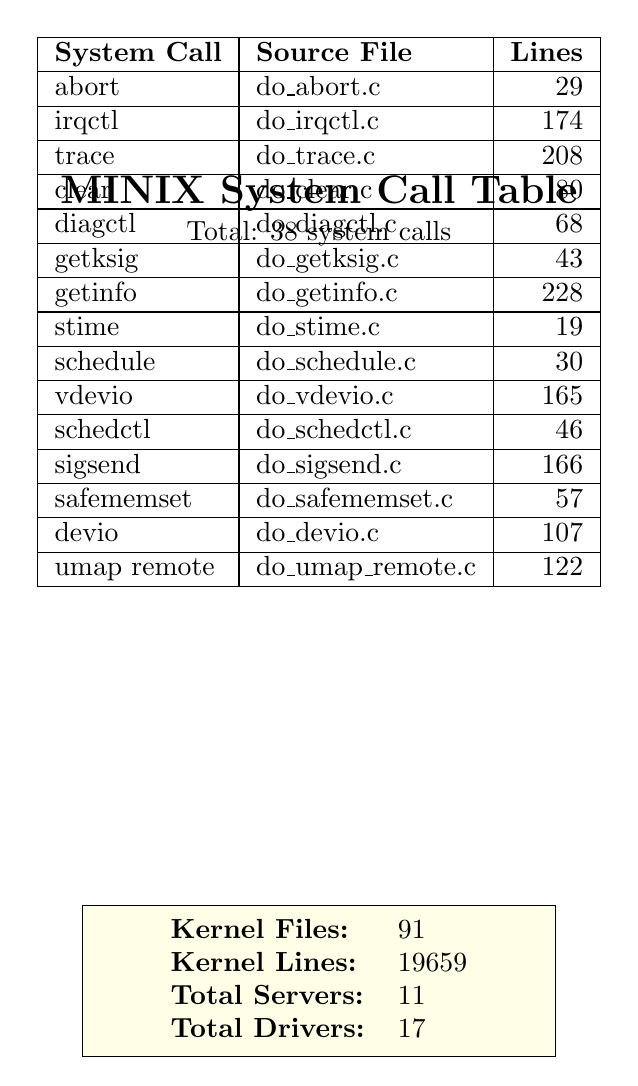
\begin{tikzpicture}

% Title
\node[font=\Large\bfseries] at (0, 0) {MINIX System Call Table};
\node[font=\normalsize] at (0, -0.5) {Total: 38 system calls};

% Create table
\node at (0, -1.5) {
\begin{tabular}{|l|l|r|}
\hline
\textbf{System Call} & \textbf{Source File} & \textbf{Lines} \\
\hline
abort & do\_abort.c & 29 \\
\hline
irqctl & do\_irqctl.c & 174 \\
\hline
trace & do\_trace.c & 208 \\
\hline
clear & do\_clear.c & 80 \\
\hline
diagctl & do\_diagctl.c & 68 \\
\hline
getksig & do\_getksig.c & 43 \\
\hline
getinfo & do\_getinfo.c & 228 \\
\hline
stime & do\_stime.c & 19 \\
\hline
schedule & do\_schedule.c & 30 \\
\hline
vdevio & do\_vdevio.c & 165 \\
\hline
schedctl & do\_schedctl.c & 46 \\
\hline
sigsend & do\_sigsend.c & 166 \\
\hline
safememset & do\_safememset.c & 57 \\
\hline
devio & do\_devio.c & 107 \\
\hline
umap remote & do\_umap\_remote.c & 122 \\
\hline
\end{tabular}
};

% Statistics box
\node[draw=black, fill=yellow!10, minimum width=6cm, minimum height=1.5cm] at (0, -10) {
\begin{tabular}{ll}
\textbf{Kernel Files:} & 91 \\
\textbf{Kernel Lines:} & 19659 \\
\textbf{Total Servers:} & 11 \\
\textbf{Total Drivers:} & 17
\end{tabular}
};

\end{tikzpicture}
\end{document}